\documentclass[10pt,a4paper,titlepage]{report}
\usepackage[utf8]{inputenc}
\usepackage{amsmath}
\usepackage{amsfonts}
\usepackage{amssymb}
\usepackage{graphicx}
\usepackage{xcolor}
\usepackage{minted}

\newcommand{\HRule}[1]{\rule{\linewidth}{#1}}

\nonstopmode


\begin{document}
{\fontfamily{cmr}\selectfont
\title{ \normalsize \textsc{}
\\ [2.0cm]
\HRule{0.5pt} \\
\LARGE \textbf{\uppercase{Functions and Procedures}
\HRule{2pt} \\ [0.5cm]
\normalsize \today \vspace*{5\baselineskip}}
}

\date{}

\author{
	Rwithik Manoj \\
	College of Engineering, Trivandrum \\
	Department of Computer Science and Engineering }

\maketitle
\newpage

\sectionfont{\scshape}

}
\begin{enumerate}
	\item Create a function factorial to find the factorial of a number. Use this function in a PL/pgSQL Program to display the factorial of a number.
	\begin{verbatim}
CREATE OR REPLACE FUNCTION factorial(n INTEGER)
RETURNS INTEGER AS
$$
DECLARE
	fact INTEGER := 1;
BEGIN
	IF n < 1 THEN
		RETURN 1;
	END IF;
	FOR i IN 1..n LOOP
		fact := fact * i;
	END LOOP;
	RAISE NOTICE 'Factorial is %', fact;
	RETURN fact;
END;
$$ LANGUAGE plpgsql;
	\end{verbatim}
	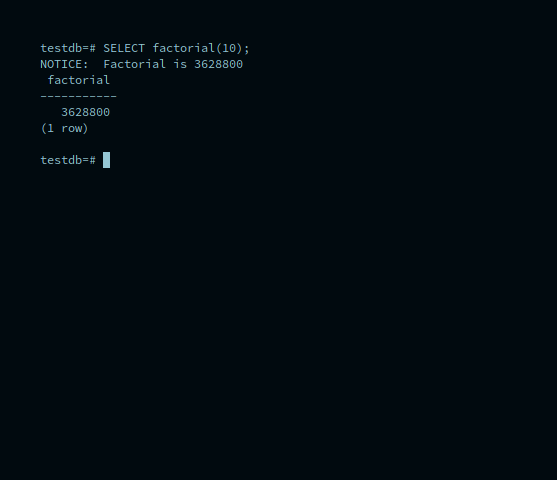
\includegraphics[width=\linewidth]{../Images/Functions/1.png}

	\item Create a table student\_details(roll int, marks int, phone int). Create a procedure pr1 toupdate all rows in the database. Boost the marks of all students by 5\%.
	\begin{verbatim}
CREATE OR REPLACE FUNCTION grading()
RETURNS INTEGER
AS $$
DECLARE
t INTEGER := 0
cur CURSOR FOR SELECT * FROM student
rec RECORD
grd CHAR(1)
BEGIN
OPEN cur
LOOP
t := 0
FETCH cur into rec
EXIT WHEN NOT FOUND
t := rec.m1 + rec.m2 + rec.m3
UPDATE student SET total = t WHERE CURRENT OF cur
IF t > 250 THEN
grd := 'A'
ELSIF t > 200 THEN
grd := 'B'
ELSIF t > 150 THEN
grd := 'C'
ELSIF t > 100 THEN
grd := 'D'
ELSE
grd := 'F'
END IF
CALL marks(rec.id, grd)
END LOOP
CLOSE cur
RETURN null
END
$$ LANGUAGE plpgsql

CREATE OR REPLACE PROCEDURE marks(tid INTEGER, tgrd CHAR)
LANGUAGE plpgsql
AS $$
BEGIN
UPDATE studentmark SET grade=tgrade WHERE id=tid
END
$$;
	\end{verbatim}
	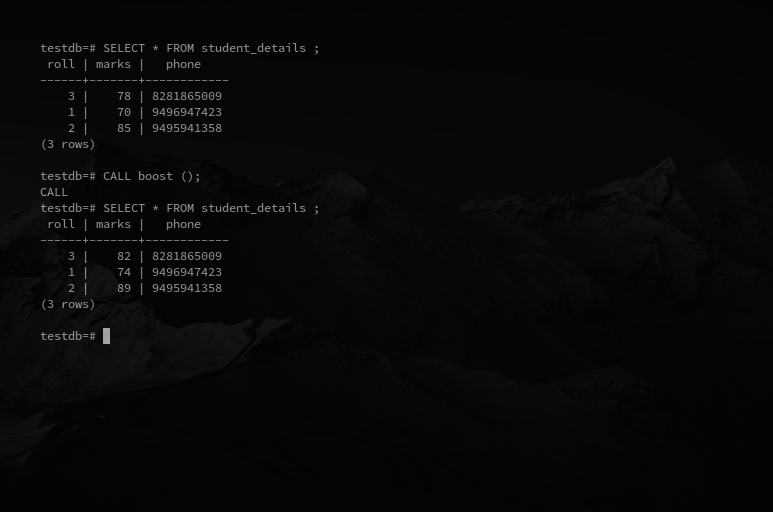
\includegraphics[width=\linewidth]{../Images/Functions/2.png}

	\item Create table student (id, name, m1, m2, m3, total, grade).Create a function f1 to calculate grade. Create a procedure p1 to update the total and grade.\newline
Using a function to calculate the grade.\newline
Using a procedure to update the grade value for the tuple.\newline
	\begin{verbatim}
CREATE OR REPLACE FUNCTION grading()
RETURNS INTEGER
AS $$
DECLARE
	t INTEGER := 0;
	cur CURSOR FOR SELECT * FROM student;
	rec RECORD;
	grd CHAR(1);
BEGIN
	OPEN cur;
	LOOP
		t := 0;
		FETCH cur into rec;
		EXIT WHEN NOT FOUND;
		t := rec.m1 + rec.m2 + rec.m3;
		UPDATE student SET total = t WHERE CURRENT OF cur;
		IF t > 250 THEN
			grd := 'A';
		ELSIF t > 200 THEN
			grd := 'B';
		ELSIF t > 150 THEN
			grd := 'C';
		ELSIF t > 100 THEN
			grd := 'D';
		ELSE
			grd := 'F';
		END IF;
		CALL marks(rec.id, grd);
	END LOOP;
	CLOSE cur;
	RETURN null;
END;
$$ LANGUAGE plpgsql;
	\end{verbatim}
	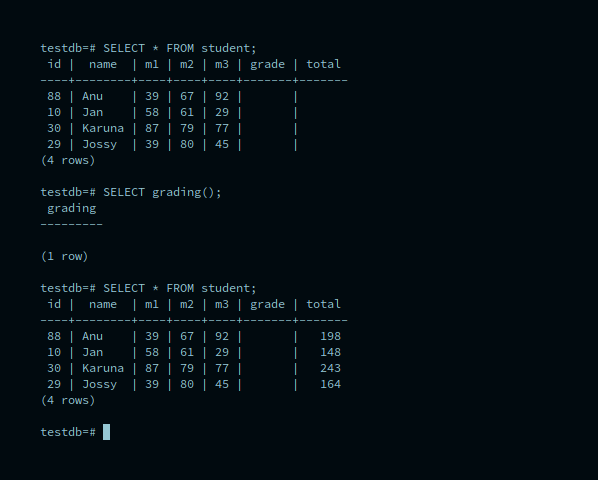
\includegraphics[width=\linewidth]{../Images/Functions/3.png}

	\item Create a package pk1 consisting of the following functions and procedures 
	\begin{enumerate}
		\item Procedure proc1 to find the sum, average and product of two numbers 
		\item Procedure proc2 to find the square root of a number 
		\item Function named fn11 to check whether a number is even or not
		\item A function named fn22 to find the sum of 3 numbers 
	\end{enumerate}
		Use this package in a PL/SQL program. Call the functions f11, f22 and procedures pro1, pro2 within the program and display their results.
\end{enumerate}

\begin{verbatim}

CREATE SCHEMA pk1

CREATE OR REPLACE PROCEDURE pk1.proc1(num1 REAL,num2 REAL)
LANGUAGE plpgsql
AS
$$
DECLARE
sum REAL
average REAL
prod REAL
BEGIN
sum = num1 + num2
prod = num1 * num2
average = (num1 + num2) / 2
RAISE NOTICE 'Sum of % and % is %', num1, num2, sum
RAISE NOTICE 'Product of % and % is %', num1, num2, prod
RAISE NOTICE 'Average of % and % is %', num1, num2, average
END
$$

CREATE OR REPLACE PROCEDURE pk1.proc2(num1 REAL)
LANGUAGE plpgsql
AS
$$
DECLARE
root REAL
BEGIN
root = sqrt(num1)
RAISE NOTICE 'Root of % is %', num1, root
END
$$

CREATE OR REPLACE FUNCTION pk1.fn11(num REAL) RETURNS VOID AS
$$
DECLARE
rem INT 
BEGIN
rem = num
rem = rem %2
IF rem = 1 THEN
	RAISE NOTICE 'Number % is odd', num
	ELSE
		RAISE NOTICE 'Number % is even', num
		END IF
		END
		$$ LANGUAGE plpgsql

		CREATE OR REPLACE FUNCTION pk1.fn22(num1 REAL, num2 REAL, num3 REAL) RETURNS VOID AS
		$$
		DECLARE
		sum REAL 
		BEGIN
		sum = num1 + num2 + num3
		RAISE NOTICE 'Sum of % , %, % is %', num1, num2, num3, sum
		END
		$$ LANGUAGE plpgsql

		CREATE OR REPLACE FUNCTION pk1.all(num1 REAL, num2 REAL, num3 REAL)
		RETURNS VOID AS
		$$
		DECLARE
		BEGIN
		CALL pk1.proc1(num1, num2)
		CALL pk1.proc2(num1)
		PERFORM pk1.fn11(num1)
		PERFORM pk1.fn22(num1, num2, num3)
		END
		$$ LANGUAGE plpgsql;
\end{verbatim}

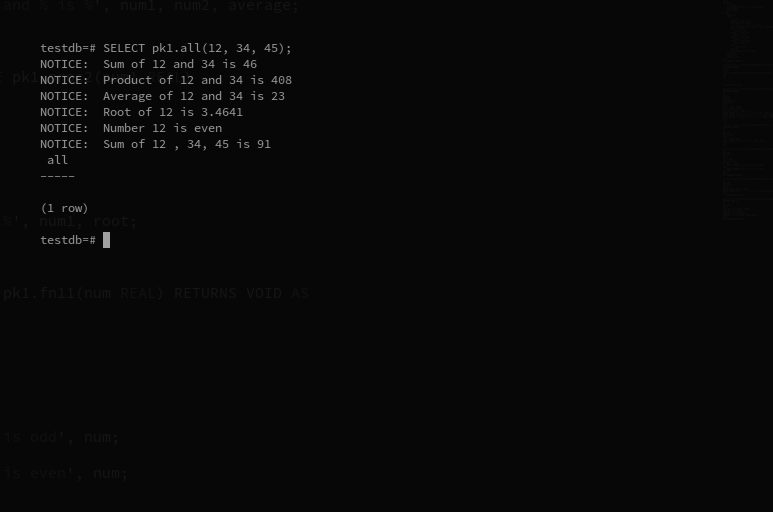
\includegraphics[width=\linewidth]{../Images/Functions/4.png}

\subsubsection{RESULT}
The PL/SQL programs were executed successfully and the output was obtained.

}
\end{document}
